\documentclass[11pt]{article}
\usepackage[a4paper, total={6in, 8in}]{geometry}
\usepackage[export]{adjustbox}
\usepackage[utf8]{inputenc}
\usepackage{hyperref}
\usepackage{graphics}
\usepackage{amssymb}
\usepackage[english]{babel}
\usepackage{amsmath}
\usepackage[classfont=bold]{complexity}
\usepackage{tikz}
\usepackage{amsthm}
\usepackage[ruled, linesnumbered, noend]{algorithm2e}
\renewcommand{\thealgocf}{}
\usetikzlibrary{arrows,automata}


\hypersetup{
    colorlinks=false
}
\urlstyle{same}
\graphicspath{ {./images/} }
\everymath{\displaystyle}

\title
{%
  {\Huge CS412 Final Project \\
  \Huge Travelling Salesman Problem\\
    \huge Implementations and Analysis of Various Solutions}
}
\date{\Large \today}
\begin{document}
\maketitle
\centering
\includegraphics[scale=0.2]{images/title.png}
\newpage
\paragraph{}
\paragraph{}
\paragraph{}
\paragraph{}
\paragraph{}
\paragraph{}
\paragraph{}
\paragraph{}
\paragraph{}
\par \centering
This page is has been intentionally left blank intentionally \paragraph{}
The typo in the sentence above is left unfixed intentionally as well, because leaving a page intentionally blank makes the same amount of sense as leaving a typo in a sentence intentionally unfixed. 
\par \flushleft

\newpage
\tableofcontents

\newpage


\newpage
\section{Introduction}
The travelling salesman problem has a long history of being a problem of interest in the field of algorithms. It has garnered much attention and there has been a lot of work that has been done on it. In this project we will set out to establish the details of this problem and why it is so tough. We will then investigate 4 algorithms that have become well known in being useful for solving this problem. One of them produces an exact solution and the rest use approximation techniques. We will be using theory and implementation to test the runtimes of this problem and will then present our research in an appropriate format.
\subsection{Proof: TSP $\in$ NP-hard}
\section{Design Techniques}
	\subsection{Exact Solution}
	The exact solution of the travelling salesman problem requires that that each Hamiltonian cycle is travelled and the minimum path of those cycles is found. However, this is an extremely large problem as there will be $n!$ cycles for a complete graph of size $n$. The dynamic programming approach called the Held-Karp algorithm reduces this time complexity to $O(n^22^n)$. It does so by dividing the problem into sub problems.  A very simple method is to visulize this idea using a tree. \paragraph{}
	Let us begin this explanation, without loss of generality, with a complete graph, $K_4,$ that does not contain loops. 
\begin{center}
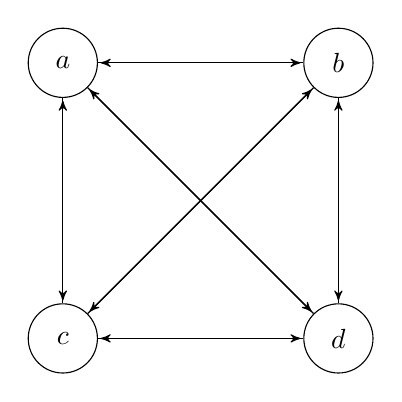
\begin{tikzpicture}[->,>=stealth',shorten >=1pt,auto,node distance=3.5cm,scale = 1,transform shape]

  \node[state] (a) [] {$a$};
  \node[state] (b) [right of=a] {$b$};
  \node[state] (c) [below of=a] {$c$};
  \node[state] (d) [below of=b] {$d$};

  \path (a) edge              node {} (b)
        (b) edge              node {} (a)
        (a) edge              node {} (c)
        (c) edge              node {} (a)
        (a) edge              node {} (d)
        (d) edge              node {} (a)
        (b) edge              node {} (c)
        (c) edge              node {} (b)
        (b) edge              node {} (d)
        (d) edge              node {} (b)
        (c) edge              node {} (d)
        (d) edge              node {} (c);

\end{tikzpicture}
\end{center}
Starting from vertex a, or any vertex to maintain generality, we can build a decision tree that traverses each path, this represents the the power set of the graph
\begin{center}
    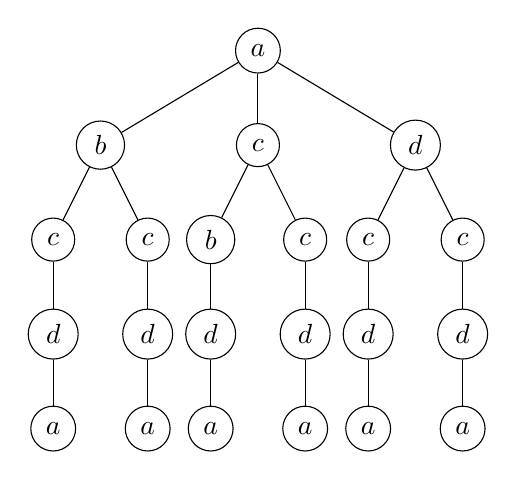
\begin{tikzpicture}[sibling distance=10em,
  every node/.style = {shape=circle, rounded corners,
    draw, align=center,
    top color=white, bottom color=white!5}, scale=0.8]
    \tikzstyle{level 1}=[sibling distance=25mm] 
    \tikzstyle{level 2}=[sibling distance=15mm] 
    \tikzstyle{level 3}=[sibling distance=10mm] 
    
  \node {$a$}
    child { node {$b$} 
        child {node {$c$}
        child {node {$d$}
        child {node {$a$}}}}
        child {node {$c$}
        child {node {$d$}
        child {node {$a$}}}}}
    child { node {$c$} 
        child {node {$b$}
        child {node {$d$}
        child {node {$a$}}}}
        child {node {$c$}
        child {node {$d$}
        child {node {$a$}}}}}
    child { node {$d$} 
        child {node {$c$}
        child {node {$d$}
        child {node {$a$}}}}
        child {node {$c$}
        child {node {$d$}
        child {node {$a$}}}}};
\end{tikzpicture}
\end{center}
The idea behind the exhaustive, brute-force approach is to traverse each path in the tree and then decide, this creates a very large problem to solve. The idea behind the dynamic approach is to start from the level 4 of the tree, which means we are now at the last vertex in the path and the next vertex from that completes the cycle and takes us back to the source node. This forms the smallest sub problem in the dynamic program. The next step would be go a level higher in the tree, which means we will now check the path length if we are reaching the source node from vertex $v$ and, we are reaching reaching vertex, $v$, from vertex, $u$ s.t. $u,v \in V$ where $V$ is the set of all vertices. We will keep doing this, and at each level we will decide the minimum path length of between n paths that are emerging from one vertex, this is done until the source node of the tree is reached, resulting in the minimum path. The dynamic algorithm can be generalised as a cost function, $g$, as follows:
$$g(i, S) = min_{k\in S} \bigg\{c_{ik} + g(k, S-\{k\})\bigg\}$$
s.t. $i$ is the source vertex, $S$ is the set of all vertices, $c_{ik}$ is the cost of some going from vertex $i$ to $k$. 
	
\subsubsection{Held-Karp Algorithm}
		
		
		
	\subsection{ Approximate Solutions}
		\subsubsection {Nearest Neighbour Algorithm}
    \subsubsection {Pairwise Exchange Method}
    \newpage
    \subsubsection {Christofides–Serdyukov Algorithm}
    The Christofides–Serdyukov algorithm is another approximation algorithm, that gives a solution that is 
    relatively close to the optimal TSP tour. First, we will take a look at a simpler approximation 
    algorithm that results in an approximation ratio of 2.

    \begin{algorithm*}
      \KwIn{A weighted complete graph $G$ and a root vertex $v$}
      \KwOut{A hamiltonian cycle $H$.}
      compute a minimum spanning tree $T$ for $G$ using \textsc{MST-PRIM}($G, v$) \\
      let $H$ be the list of vertices, ordered according to when they are first visited in a
      preorder tree walk of $T$ \\
      \Return{\upshape the hamiltonian cycle $H$}
  \caption{\textsc{approx-tsp-tour}}
  \end{algorithm*}
    
  This algorithm relies on the assumption that the weights of the edges of the graph conform to the triangle inequality and that the graph is complete.
  Let $c(u,v)$ be the weight of 
  an edge. Then, \[c(u,w) \leq c(u,v) + c(v, w) \]
  In simpler words, removing an intermediate stop would never increase the cost. If the edges do not conform to the triangle inequality, then a polynomial-time approximation
  with a constant approximation ratio does not exist, unless $\P = \NP$. The proof of this
  is outside the scope of this paper. This version of the TSP is also called a metric TSP since 
  the edge weights form a metric space.   
  \paragraph{} Let's look at a short proof that \textsc{approx-tsp-tour} is a poly-time 2- approximation algorithm. 
  \begin{proof}
    Let $H^*$ denote the optimal TSP tour for a set of vertices. We can obtain a spanning tree $T$ by eliminating an edge from 
    $H^*$. This provides a lower bound for cost of $H*$. 
    \[c(T) \leq c(H^*)\] A full walk $W$ of $T$ would visit every edge of $T$ twice, which means   
    \[c(W) = 2\cdot c(T) \implies c(W) \leq 2\cdot c(H^*)\]
  Since, the triangle inequality is being obeyed, we can remove repeated visits in $W$ with a guarantee that 
  the cost will not increase.
  Let $H$ be the cycle corresponding to a pre-order walk in $T$. This hamiltonian cycle is the cycle that is computed by 
  \textsc{approx-tsp-tour}. Since $H$ is obtained by deleting vertices from $W$,
  \[c(H) \leq c(W)\]
  This implies that, \[c(H) \leq 2\cdot c(H^*)\] which completes the proof. 
  \end{proof}

  \textbf{An Improved Algorithm:}  \paragraph{}
  
  This algorithm can be improved by adding a few more graph operations that can further optimize our solution.
  The improved algorithm by Christofides relies on the same assumptions (triangle inequality and complete graph). 
  However, it utilizes other graph properties to improve the approximation ratio. These facts/properties are:
  \begin{enumerate}
    \item The number of vertices with odd degree in a graph is always even, according to the handshaking lemma. 
    \item A graph that has all vertices with even degree will have an Eulerian tour. 
    \item Given a complete weighted graph, 
  \end{enumerate}  
  
  
\section{Theoretical Runtime Analysis and Comparison}
\section{Empirical Runtime Analysis and Comparison}
\section{Conclusion}
\newpage
\section{References}
\begin{enumerate}
	\item \url{https://www.researchgate.net/publication/289195926_On_the_Nearest_Neighbor_Algorithms_for_the_Traveling_Salesman_Problem}
	\item \url{https://en.wikipedia.org/wiki/Travelling_salesman_problem#:~:text=The%20travelling%20salesman%20problem%20}
	\item Thomas H. Cormen, Charles E. Leiserson, Ronald L. Rivest, and Clifford Stein. 2009. Introduction to Algorithms, Third Edition (3rd. ed.)
	\item David L. Applegate, Robert E. Bixby, Vasek Chvatal, and William J. Cook. 2007. The Traveling Salesman Problem: A Computational Study. Princeton University Press, USA.
\end{enumerate}




\end{document}